\documentclass[11pt]{article}

\usepackage[T1]{fontenc}
\usepackage[margin=1in]{geometry}
\usepackage{times}
\usepackage{url}
\usepackage{hyperref}
\usepackage{graphicx}
\usepackage{array}
\usepackage{tabularx}
\usepackage{booktabs}
\usepackage{enumitem}
\usepackage{amsmath}
\usepackage{tikz}
\usetikzlibrary{arrows.meta, positioning, shapes.geometric, fit, calc}

\hypersetup{
  colorlinks=true,
  linkcolor=blue,
  citecolor=blue,
  urlcolor=blue
}

\setlist[itemize]{leftmargin=*}
\setlist[enumerate]{leftmargin=*}
\sloppy
\newcommand{\mcnemar}[3]{\mbox{\(+#1/-#2,\;p=#3\)}}
\newcommand{\cfgflag}[2]{\mbox{\texttt{#1 = #2}}}

\title{Graph-Conditioned Neural Decompilation of Dart AOT Binaries: Architecture, Functional Evaluation, and a Leakage Audit}
\author{Raafat Abualazm \and Ayman AboElHassan \and Amr G. Wassal}
\date{}

\begin{document}
\maketitle

\begin{abstract}
Neural decompilation is increasingly framed as code generation, but surface similarity and syntactic validity can diverge sharply from functional correctness. We implement a graph-conditioned Dart AOT decompiler in which GraphCodeBERT encodes bounded assembly blocks, a typed four-layer GINE propagates CFG/DFG information, global block attention aggregates the sequence, and learned query tokens resample it into a gated prefix for a Qwen3-8B decoder. We also study GRPO, rejection-sampling fine-tuning, reranking, and candidate pooling.

An audit of the released artifact found a material defect in the historical local functional evaluation: the local prompt builder copied assertions from the same unit-test harness later used for pass@k, including concrete expected outputs. Those local pass@k, pass-set compile@k, reward-adaptation, repair, reranking, and union pools are therefore test-informed and are withdrawn as hidden-test evidence. The ordinary 1,195-row SFT corpus and separate 126-row CodeBLEU corpus contain no scoring-test field and are not affected by this specific leak. Hosted frontier pools were generated by separate test-free prompt builders; their absolute zero-shot results remain informative, but comparison with the historical local pools is not information-matched. We contribute the corrected protocol and implementation: a test-free prompt schema, physically disjoint GRPO train/evaluation files, source-grouped SFT splits, stable evaluator task IDs, immutable model revisions, run-level hashes and seeds, and controlled no-edge, shuffled-edge, CFG-only, CFG+DFG, and no-GINE ablations. Until those multi-seed runs complete, this document is an audited experimental design and historical diagnostic, not a claim of clean local functional superiority.
\end{abstract}

\begin{center}
\fbox{\parbox{0.94\linewidth}{\textbf{Correction status (July 10, 2026).}
Historical local 154-task functional results in this draft are contaminated by
scoring-test assertions in the policy prompt. They are retained only to document
the audit and are not submission-ready evidence. A leakage-free multi-seed rerun
is required before the local architecture, GRPO, or ensemble claims can be made.}}
\end{center}

\noindent\textbf{Index Terms}--Neural decompilation, reverse engineering, Dart AOT, graph-conditioned code models, pass@k, CodeBLEU, reinforcement learning, reranking.

\section{Introduction}

Decompilation reconstructs high-level source-like programs from low-level binaries. For reverse engineering, malware analysis, security auditing, and software maintenance, the useful output is not merely compilable pseudocode. It should be readable, idiomatic, and functionally faithful to the original program. Traditional decompilers recover valuable control and data-flow information, but their outputs often contain generic identifiers, low-level control structures, and C-like artifacts that are far from the original source language.

Neural decompilation treats this recovery problem as translation or code generation. Katz et al. showed that sequence models can learn some assembly-to-source patterns, but their RNN setting predates modern code LLMs and focuses on small C-like snippets \cite{katz2018rnn}. DIRE and DIRTY then shifted attention to a key missing artifact in decompiler output: meaningful variable names and types \cite{lacomis2019dire,chen2022dirty}. SLaDe and LLM4Decompile moved closer to end-to-end neural decompilation, showing that Transformer and LLM systems can improve readability and re-executability for C-family binaries \cite{armengol2023slade,tan2024llm4decompile}. Recent systems including CFADecLLM, HELIOS, SALT4Decompile, SK2Decompile, AutoDecompiler, and Nova make structure-aware and feedback-driven LLM decompilation an active direction \cite{liu2025cfadecllm,achamyeleh2026helios,wang2025salt4decompile,tan2025sk2decompile,liu2026autodecompiler,jiang2025nova}. They do not settle the managed-language case. Dart is especially challenging: production Flutter applications are compiled Ahead-of-Time (AOT), and the resulting native code reflects type specialization, inlining, and runtime-specific object representations.

Prior Dart-focused work showed that small specialized models can generate readable Dart and can approach much larger code models on CodeBLEU under limited-data conditions \cite{abualazm2026idiomatic}. The follow-up HumanEval-Dart study showed why that result is not enough: fine-tuning can improve CodeBLEU and compile@k while failing to improve, or even regressing, pass@k functional correctness \cite{abualazm2026tosem}. This paper is the architectural and selection-oriented extension of those studies: the earlier work established the target and metric mismatch, while this work tests graph-conditioned decoding, reward adaptation, and candidate selection against pass@k. We therefore treat functional correctness as the central evaluation target and use CodeBLEU and compile@k as diagnostic metrics rather than final evidence of decompilation success.

Motivated by the finding that sequence-only fine-tuning does not reliably improve functional correctness, we evaluate whether graph-conditioned decoding, reward adaptation, reranking, and candidate pooling recover additional semantic fidelity. We investigate two complementary ideas. First, decompilation is not plain text translation: assembly has explicit control-flow and data-flow structure. We therefore condition a causal decoder on graph-derived representations built from extracted basic blocks, control-flow edges, and lightweight data-flow edges. Second, pass@k is a tail metric: it rewards the existence of at least one correct candidate among many. A single checkpoint optimized for expected per-sample reward may narrow its output distribution and reduce the diversity needed for pass@k. We therefore distinguish single-model performance from multi-arm candidate coverage and reranking. Throughout, we anchor these specialized-model results against strong general-purpose frontier models prompted zero-shot on the same assembly, so that every specialized number is read against the capability a practitioner could obtain today by calling a hosted model.

The corrected study is organized around four questions. \textbf{RQ1} asks whether graph topology improves a local 8B model when block encoder, prefix adapter, prompt, parameterization, and candidate budget are fixed. \textbf{RQ2} asks whether GRPO improves held-out tasks when tests remain private to the reward process and training/evaluation tasks are disjoint. \textbf{RQ3} calibrates leakage-free local models against hosted frontier capability under matched visible information. \textbf{RQ4} asks whether complementary policies improve coverage at a fixed total candidate budget. The historical pools below motivated these questions but cannot answer them because of the disclosed leakage and provenance gaps.

The test-free hosted pools still establish a useful practitioner reference: on the 154-task set, the July 8, 2026 GPT-5.5 snapshot reaches pass@10 of 0.701, and controlled prompt-representation ablations do not show a significant benefit from textual CFG serialization. Those results do not validate the old local comparison. The current contribution is therefore narrower: an implemented latent graph-prefix architecture, an explicit account of why its first functional evaluation is invalid, and a reproducible confirmatory protocol. We report the historical local tables only as contaminated diagnostics so that the failure is visible rather than silently erased.

\section{Related Work}

\subsection{Neural decompilation and binary-to-source recovery}

Katz et al. framed neural decompilation as sequence-to-sequence recovery from binary code to source-like text \cite{katz2018rnn}. Their result is important because it showed that learned models can replace some hand-engineered decompiler stages, but it also exposed the limits of flat sequence modeling. DIRE and DIRTY address a different part of the information-loss problem: they recover identifiers and types for decompiler output rather than generating a complete source program from assembly \cite{lacomis2019dire,chen2022dirty}. ReSym pushes that direction further by combining LLMs with program analysis to recover variable and data-structure symbols from stripped binaries \cite{xie2024resym}. These works motivate learned semantic recovery, but they assume C/C++-oriented artifacts and do not model Dart AOT runtime conventions.

More recent systems attempt end-to-end assembly-to-C recovery. Beyond the C argues for retargetable neural translation rather than language-specific decompiler engineering \cite{hosseini2022beyondc}. SLaDe pairs a portable small language model with type inference, and LLM4Decompile scales open LLMs over assembly/source corpora \cite{armengol2023slade,tan2024llm4decompile}. CFADecLLM injects control-flow information into an end-to-end decompiler; HELIOS serializes hierarchical CFG/call structure for general LLMs; SALT4Decompile reconstructs a source-level abstract logic tree; and Nova learns hierarchical assembly representations \cite{liu2025cfadecllm,achamyeleh2026helios,wang2025salt4decompile,jiang2025nova}. SK2Decompile separates structural and identifier recovery, while AutoDecompiler uses compiler, execution, and test feedback for multi-turn refinement \cite{tan2025sk2decompile,liu2026autodecompiler}. These systems make clear that neither structural conditioning nor reward feedback is itself novel. Our narrower target is Dart AOT and a latent block-graph-to-prefix adapter, coupled with an explicit audit of pass@k protocol integrity. Decompile-Bench expands the field with million-scale binary-source pairs, while Idioms studies joint code and type recovery \cite{tan2025decompilebench,dramko2025idioms}.

Existing Dart and Flutter reverse-engineering tools occupy a different point in the design space. Tools such as B(l)utter, reFlutter, and JEB's Dart AOT snapshot helper focus on snapshot introspection, runtime patching, metadata recovery, or analyst assistance for Flutter applications \cite{blutter,reflutter,jebdartaot}. They are important operational baselines for Dart reverse engineering, but they do not attempt the same source-level, test-executed neural decompilation task studied here.

\subsection{Code metrics and functional correctness}

CodeBLEU was designed to improve over lexical BLEU by adding syntax and data-flow components \cite{ren2020codebleu}. That makes it a better similarity metric for code, but it still measures agreement with a reference rather than executable behavior. HumanEval introduced pass@k as a functional code-generation metric: the question is whether at least one of k sampled programs passes tests \cite{chen2021codex}. MultiPL-E established a scalable method for translating HumanEval and MBPP into 18 additional languages, but its original benchmark did not include Dart \cite{cassano2023multiple}. HumanEval-Dart is our separate Dart-specific adaptation of that unit-test translation paradigm, paired here with Dart AOT assembly and graph artifacts for decompilation. The earlier Dart AOT metric study connected these lines and showed that CodeBLEU, compile@k, and pass@k can move in different directions on neural decompilation \cite{abualazm2026tosem}. We therefore report CodeBLEU and compile@k, but we interpret them as supporting diagnostics. pass@k and task-level coverage are the main evidence for semantic recovery.

\subsection{Candidate selection and reranking}

Candidate selection has a long precedent in code generation. AlphaCode generated large pools of programs, filtered them, clustered similar solutions, and selected a small submission set for programming-contest problems \cite{li2022alphacode}. Our compile-cluster reranker uses the same broad filter-and-cluster philosophy, but in a different setting: decompilation from assembly to Dart, where hidden tests cannot be used by a deployable selector. We therefore separate deployable compile-aware reranking from oracle reranking, which is reported only as an upper bound on candidate-pool quality.

\subsection{Graph-conditioned code modeling}

GraphCodeBERT demonstrates that data-flow structure can improve code representations over flat token sequences \cite{guo2020graphcodebert}. We use the same principle in a different direction: GraphCodeBERT encodes assembly within each block, while typed GINE layers consume cross-block CFG/DFG edges and a learned resampler conditions the generator. CFADecLLM and HELIOS are the closest control-flow-aware comparisons, SALT4Decompile is the closest recovered-logic abstraction, and AutoDecompiler is the closest reward-feedback comparison \cite{liu2025cfadecllm,achamyeleh2026helios,wang2025salt4decompile,liu2026autodecompiler}. The remaining distinction is the latent graph-prefix path for a small private Dart AOT model, not a claim that structure-aware decompilation is new.

\subsection{Adaptation and preference optimization}

LoRA makes these experiments feasible by adapting large pretrained models with low-rank trainable updates instead of full fine-tuning \cite{hu2021lora}. We apply LoRA to both GraphCodeBERT and Qwen3; the corrected runs pin \texttt{Qwen/Qwen3-8B}, while historical base identity remains unresolved \cite{yang2025qwen3}. For reward adaptation, we implement GRPO, introduced by DeepSeekMath as a critic-free group-relative variant of PPO \cite{shao2024deepseekmath}. SimPO motivates simple sequence-level preference objectives, while SimKO directly targets pass@K concentration in RLVR \cite{meng2024simpo,peng2025simko}. Recent RLVR analyses likewise motivate measuring pass@1, pass@k, and diversity separately \cite{yue2025rlvr}. Whether those dynamics improve decompilation is a question for the clean held-out rerun, not a conclusion from the contaminated historical arm.

\section{Method}

\begin{figure}[t]
\centering
\resizebox{\textwidth}{!}{%
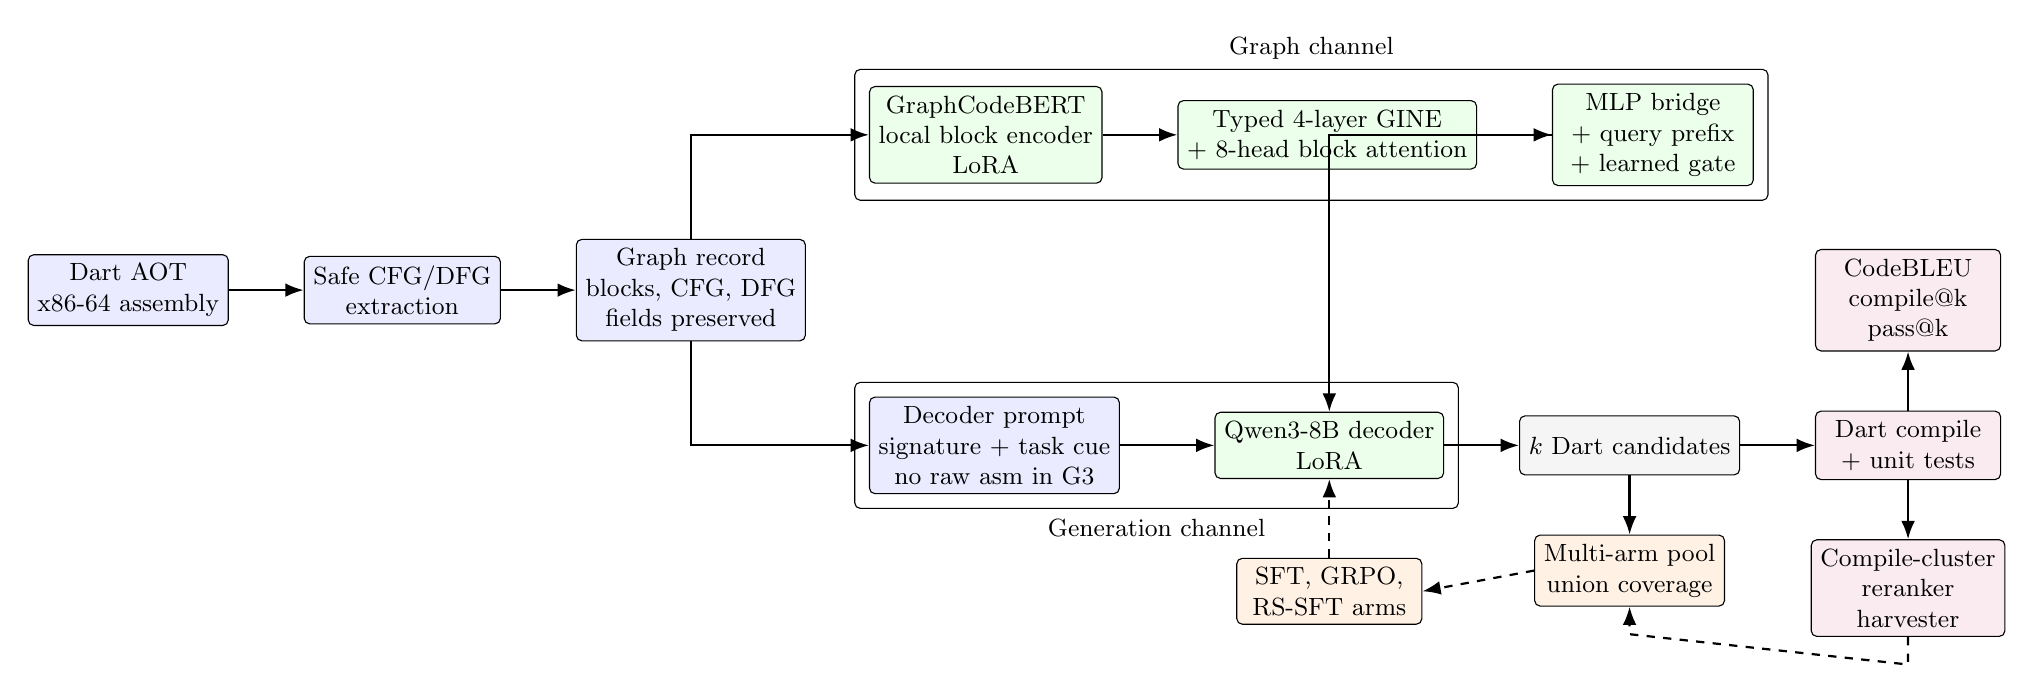
\begin{tikzpicture}[
  font=\small,
  >=Latex,
  node distance=0.75cm and 0.95cm,
  box/.style={draw, rounded corners=2pt, align=center, minimum height=0.75cm, minimum width=2.2cm, fill=gray!8},
  data/.style={draw, rounded corners=2pt, align=center, minimum height=0.75cm, minimum width=2.35cm, fill=blue!8},
  model/.style={draw, rounded corners=2pt, align=center, minimum height=0.82cm, minimum width=2.55cm, fill=green!8},
  train/.style={draw, rounded corners=2pt, align=center, minimum height=0.75cm, minimum width=2.35cm, fill=orange!10},
  eval/.style={draw, rounded corners=2pt, align=center, minimum height=0.75cm, minimum width=2.35cm, fill=purple!8},
  arrow/.style={->, thick},
  dasharrow/.style={->, thick, dashed}
]

\node[data] (asm) {Dart AOT\\x86-64 assembly};
\node[data, right=of asm] (extract) {Safe CFG/DFG\\extraction};
\node[data, right=of extract] (graph) {Graph record\\blocks, CFG, DFG\\fields preserved};

\node[model, above right=0.7cm and 0.8cm of graph] (encoder) {GraphCodeBERT\\local block encoder\\LoRA};
\node[model, right=of encoder] (message) {Typed 4-layer GINE\\+ 8-head block attention};
\node[model, right=of message] (pool) {MLP bridge\\+ query prefix\\+ learned gate};

\node[data, below right=0.7cm and 0.8cm of graph] (prompt) {Decoder prompt\\signature + task cue\\no raw asm in G3};
\node[model, right=1.2cm of prompt] (decoder) {Qwen3-8B decoder\\LoRA};
\node[box, right=of decoder] (cands) {$k$ Dart candidates};

\node[eval, right=of cands] (harness) {Dart compile\\+ unit tests};
\node[eval, above=of harness] (metrics) {CodeBLEU\\compile@k\\pass@k};
\node[eval, below=of harness] (rerank) {Compile-cluster\\reranker\\harvester};

\node[train, below=1.0cm of decoder] (adapt) {SFT, GRPO,\\RS-SFT arms};
\node[train, below=of cands] (ensemble) {Multi-arm pool\\union coverage};

\draw[arrow] (asm) -- (extract);
\draw[arrow] (extract) -- (graph);
\draw[arrow] (graph) |- (encoder);
\draw[arrow] (encoder) -- (message);
\draw[arrow] (message) -- (pool);
\draw[arrow] (pool) -| (decoder);
\draw[arrow] (graph) |- (prompt);
\draw[arrow] (prompt) -- (decoder);
\draw[arrow] (decoder) -- (cands);
\draw[arrow] (cands) -- (harness);
\draw[arrow] (harness) -- (metrics);
\draw[arrow] (harness) -- (rerank);
\draw[arrow] (cands) -- (ensemble);
\draw[dasharrow] (ensemble.west) -- (adapt.east);
\draw[dasharrow] (adapt) -- (decoder);
\coordinate (rerankDrop) at ($(rerank.south)+(0,-0.35)$);
\coordinate (ensembleDrop) at ($(ensemble.south)+(0,-0.35)$);
\draw[dasharrow] (rerank.south) -- (rerankDrop) -- (ensembleDrop) -- (ensemble.south);

\node[draw, rounded corners=2pt, fit=(encoder) (message) (pool), inner sep=0.18cm, label={[font=\small]above:Graph channel}] {};
\node[draw, rounded corners=2pt, fit=(prompt) (decoder), inner sep=0.18cm, label={[font=\small]below:Generation channel}] {};
\end{tikzpicture}%
}
\caption{Corrected architecture and information boundary. GraphCodeBERT encodes bounded instructions locally; typed GINE layers propagate CFG/DFG information; global block attention and an MLP bridge feed a learned-query prefix resampler and gate. Scoring tests are available only to the evaluator and GRPO reward process, never to the policy prompt.}
\label{fig:architecture}
\end{figure}

Figure~\ref{fig:architecture} summarizes the architecture and evaluation loop. The key design choice is to avoid treating the assembly listing as another long decoder prompt. G3 is not a topology-only model: the graph/local block encoder consumes bounded per-block assembly instructions together with CFG/DFG relationships, compresses them into learned prefix tokens, and leaves only the function-level task cue in the causal decoder prompt.

\subsection{Task and data}

The study contains two historically distinct corpora, not a 126-task subset of HumanEval-Dart. The primary functional corpus has 154 filtered, test-equipped HumanEval-Dart functions with signatures, reference Dart implementations, AOT-derived x86-64 assembly, CFG/DFG-derived graph features, and unit tests. The older 126-row corpus contains standalone Dart programs and reference sources from the earlier CodeBLEU/standalone-compile workflow; its rows are mostly top-level \texttt{main} programs, do not contain the HumanEval test field, and share no filenames with the 154-task corpus. The 1,195-row ordinary SFT corpus likewise has no \texttt{tests} field. An exact and normalized token-7-gram overlap audit finds no match between that SFT corpus and the 154-task benchmark at Jaccard 0.8. Its 188 duplicate rows are grouped before the corrected 1,081/114 train-validation split.

\paragraph{Disclosed evaluation leak.} The historical local prompt builder selected up to ten lines containing \texttt{candidate} from each benchmark row's \texttt{tests} field and inserted them before the assembly. These lines include expected outputs. The pass evaluator later executed the same tests. Because prompt fitting preserved the fixed prefix and truncated assembly, test examples could be retained preferentially. All historical local 154-task functional candidate pools are therefore contaminated. The corrected prompt schema never reads \texttt{tests}; those tests are available only to the evaluator and, for GRPO training tasks, the external reward process. The integrity audit reports zero leaked rows across all 154 benchmark prompts.

\subsection{Graph extraction}

The graph pipeline extracts basic blocks from assembly using jump targets and fall-through structure, control-flow edges between blocks, lightweight data-flow edges tracking register/value relationships where available, and per-block instruction summaries with bounded instruction counts. The graph records are merged into the original JSONL rows without dropping fields such as \texttt{dart\_source}, \texttt{tests}, \texttt{dart\_function\_signature}, and \texttt{assembly}. This is important because earlier conversion code could create graph-only records and accidentally destroy the SFT/GRPO fields required by training and evaluation.

\subsection{Model architecture}

The implemented architecture is a GraphCodeBERT local block encoder followed by typed GINE message passing, global block attention, an MLP bridge, a learned-query prefix resampler, and a Qwen3-8B causal decoder. LoRA is applied to both pretrained encoder and decoder with rank 64 and alpha 128. Prefix RMS matching is a stability option for wide-prefix variants, not an assumed property of the archived 16-prefix G3 row.

For block \(i\), GraphCodeBERT encodes at most 24 normalized instructions into a local state \(h_i^{(0)}\). GraphCodeBERT does not itself receive the cross-block DFG in the reported \texttt{dfg\_mode=edges} path. Instead, CFG and reaching-definition DFG edges are consumed by four typed GINE layers. With edge type \(\tau(j,i)\) and learned type embedding \(e_{\tau}\), a layer has the form
\[
 h_i^{(\ell+1)}=\operatorname{LN}\!\left(h_i^{(\ell)}+
 \operatorname{MLP}_{\ell}\!\left((1+\epsilon)h_i^{(\ell)}+
 \sum_{j\in\mathcal{N}(i)}\operatorname{ReLU}(h_j^{(\ell)}+e_{\tau(j,i)})\right)\right).
\]
A residual connection returns the original block states after four hops. Eight-head self-attention then processes the padded block sequence, and an MLP projects from the 768-dimensional graph space into the Qwen hidden dimension. Sixteen learned queries cross-attend to the projected graph states; an FFN produces prefix core \(P\), and the decoder receives \(\sigma(g)P\), where \(g\) is a learned scalar gate. Optional RMS matching rescales each prefix vector to the RMS of the decoder embedding table before gating.

The corrected causal controls keep this entire block encoder, projection, prefix resampler, decoder cue, parameterization, and data split fixed while selecting no edges, a deterministic shuffled topology, CFG edges only, or CFG+DFG edges. A no-GINE control bypasses message passing while retaining global block attention and learned prefix pooling. The separate raw-assembly text arm remains a representation baseline rather than a causal graph-topology control.

The primary graph-conditioned configuration is given below. Each entry is a single runner parameter written as \texttt{key = value} in \texttt{snake\_case}, matching the released code:

\begin{table}[h]
\centering
\small
\begin{tabular}{@{}ll@{}}
\toprule
Parameter & Value \\
\midrule
\texttt{qwen\_prefix\_tokens} & \texttt{16} \\
\texttt{qwen\_prefix\_rms\_match} & \texttt{0} (for the reported 16-prefix G3 row) \\
\texttt{prompt\_assembly\_mode} & \texttt{"none"} \\
\texttt{prompt\_fit\_assembly} & \texttt{1} (inert when \texttt{prompt\_assembly\_mode = "none"}) \\
\texttt{dfg\_mode} & \texttt{"edges"} \\
\texttt{position\_scheme} & \texttt{"roberta"} \\
\texttt{auto\_cfg} & \texttt{0} \\
\texttt{max\_block\_instrs} & \texttt{24} \\
\texttt{graph\_max\_dataflow\_edges} & \texttt{4096} \\
\bottomrule
\end{tabular}
\end{table}

The \texttt{prompt\_assembly\_mode = "none"} setting is deliberate: the model receives structure through the graph channel rather than duplicating long assembly text in the decoder prompt. The RMS-matched p128r arm instead uses \texttt{qwen\_prefix\_rms\_match = 1}.

\subsection{Adaptation arms}

The historical study evaluated null and text-only controls, graph-text and CFG-only variants, a graph-only G3 architecture, wider prefixes, GRPO, RS-SFT, and repair arms. Because those functional pools are contaminated, this taxonomy is retained only to map released files. The confirmatory study is restricted to untuned, text-only, no-edge, shuffled-edge, CFG-only, CFG+DFG, no-GINE, and held-out GRPO arms.

\subsection{Reranking and ensembling}

We distinguish intra-model reranking from multi-arm candidate ensembling. Intra-model reranking generates k candidates from one checkpoint and selects one candidate with deployable heuristics. Multi-arm candidate ensembling pools candidates from multiple independently adapted checkpoints, then measures union coverage or reranks over the pool. The deployable reranker, \texttt{compile\_cluster\_vote}, uses Dart compilation, structural heuristics, and candidate clustering. It does not use hidden tests. Oracle reranking uses pass/fail outcomes only to estimate the upper bound available in a sampled candidate pool.

\section{Experimental Setup}

Historical sweep summaries name \texttt{Qwen/Qwen3-8B-Base}, whereas the corrected runner and later commands name \texttt{Qwen/Qwen3-8B}. Both repositories exist and share compatible tensor shapes, so adapter compatibility cannot recover which base weights were loaded. The historical local rows are therefore unpinned in addition to being test-informed. The confirmatory protocol fixes the decoder to \texttt{Qwen/Qwen3-8B@b968826d9c46dd6066d109eabc6255188de91218} and GraphCodeBERT to revision \texttt{2b0488a7bb0eefc7041f1bb2cad1ab26b0da269d}. Every prediction pool records the requested and resolved revision, prompt-stream hash, dataset/checkpoint/source hashes, seed, Git state, and runtime in a provenance sidecar.

The corrected 154-task evaluation uses ten samples, maximum generation length 768 tokens, decoder prompt budget 2048 tokens, LoRA rank 64, alpha 128, and 16 graph prefix tokens for prefix arms. Three independent training and generation seeds are specified. The separate 126-row CodeBLEU/legacy-compile workflow uses five samples and is not functional evidence. RMS matching is enabled only for explicitly labeled wide-prefix diagnostics.

For a task with \(n\) generated candidates and \(c\) passing candidates, pass@k follows the HumanEval estimator \(1 - \binom{n-c}{k}/\binom{n}{k}\), averaged over tasks \cite{chen2021codex}. We use the same convention for compile@k by replacing test pass with successful Dart front-end acceptance. When \(n=k\), as in pass@10 with ten samples and the historical compile@5 view with five samples, the estimator reduces to task coverage: whether at least one candidate succeeds. pass@1 and compile@1 reduce to \(c/n\) for each task before averaging.

Historical local multi-sample evaluation used stochastic decoding with temperature 0.7 and nucleus sampling \(p=0.95\). The confirmatory design repeats independent candidate generation for seeds 42, 43, and 44. It reports mean and standard deviation across seeds, task-and-seed hierarchical bootstrap intervals, and paired task coverage for the causal topology controls. GRPO trains on a physically separate 77-task file and is reported only on the 77-task held-out file. Historical full-set GRPO, RS-SFT, repair, and union values remain transductive contaminated diagnostics.

\paragraph{Frontier baseline.} We prompt four frontier models zero-shot on the same 154 tasks: an Azure \texttt{gpt-chat-latest} deployment identified by the provider as GPT-5.5, Claude Sonnet~5, DeepSeek~V4~Pro, and GLM-5.2, accessed through hosted APIs on July 8, 2026. Their separate prompt builders receive x86-64 AOT disassembly and the target signature but no unit tests or expected outputs. Each client makes ten requests per task. Empty content and request errors remain failed slots. This is a dated practitioner baseline rather than an architecture-controlled comparison. Its absolute test-free results remain valid, but comparison against the contaminated historical local pools is not information-matched; the clean rerun uses the same permitted signature-and-binary information boundary. The moving aliases and provider-side sampling remain limitations. All models are scored by the same JIT/pass harness, with task 160 keyed by stable task ID in every prediction schema.

\paragraph{GPT-5.5 prompt ablation.} We separately query the Azure GPT-5.5 deployment with seven prompt representations, ten candidates per task, an 8{,}192-token output cap, and deployment-default sampling shared by every ablation arm. The first serializer (\emph{v1}) supports full assembly, a character-estimated cap of approximately 2{,}048 assembly tokens, full assembly plus a compact CFG topology, and compact topology without block instructions. The cap applies to assembly text rather than to the total prompt; only 46/154 records have lower API-reported prompt-token counts than their full-assembly counterpart. That accounting check says which requests the heuristic changed; it is not an instruction-count threshold and should not be conflated with the local decoder's observed difficulty on long assembly. The revised serializer (\emph{v2}) removes GDB dump headers and uses the cleaned instruction stream in three matched conditions: cleaned assembly only, cleaned assembly plus an address-aligned CFG with final block instructions, and all normalized instructions organized inside their CFG blocks without a separate flat listing. The v2 conditions share the same cleaner, system prompt, Azure deployment, output cap, and deployment-default sampling, so their paired comparisons are controlled. Direct v1--v2 comparisons remain descriptive because the serializer revision also changes assembly cleaning and parts of the system prompt.

The corrected study uses one functional compile definition: the 154-task JIT/pass-harness metric computed from the same candidate-plus-hidden-tests files as pass@k. This guarantees that pass@k is nested under compile@k. CodeBLEU and the earlier 126-task standalone-compile view are historical diagnostics. The archived local functional numbers below are not conclusions; they document the contaminated pools that triggered the correction.

\section{Historical Results and Contamination Audit}

All local 154-task pass, aligned-compile, GRPO, repair, reranking, and union rows in this section were generated under the leaking prompt contract. They are printed for forensic traceability only and must not be cited as hidden-test performance. The frontier rows and GPT-5.5 prompt ablations used separate test-free prompt builders and remain valid absolute measurements. No inferential comparison between those frontier rows and the contaminated local rows is made.

\subsection{Standalone model results}

\begin{table}[t]
\centering
\small
\caption{Contaminated historical x86 8B pools. The 126-row CodeBLEU column is not affected by the test-hint bug; every 154-task pass@k column is test-informed and is not valid hidden-test evidence. Values are retained only to make the audit reproducible.}
\label{tab:standalone}
\resizebox{\textwidth}{!}{%
\begin{tabular}{lrrrr}
\toprule
Arm & CodeBLEU & pass@1 & pass@5 & pass@10 \\
\midrule
Binary-reward GRPO \texttt{(binary GRPO)} & 0.5438 & 0.0409 & 0.1280 & 0.1818 \\
Rejection-sampling SFT, all arms \texttt{(RS-SFT all-arms)} & 0.5740 & 0.0474 & 0.1296 & 0.1688 \\
Rejection-sampling SFT, reference \texttt{(binary RS-SFT ref)} & 0.5323 & 0.0357 & 0.1121 & 0.1558 \\
Graph-conditioned (16 prefix) \texttt{(historical G3)} & 0.6383 & 0.0266 & 0.0996 & 0.1558 \\
Style-SFT repair \texttt{(style repair ultralite)} & 0.5299 & 0.0240 & 0.0918 & 0.1429 \\
Graph-conditioned, 128 prefix + RMS \texttt{(G3 p128r)} & 0.6349 & 0.0292 & 0.0878 & 0.1364 \\
Style-SFT (1{,}036 ex.) \texttt{(style1036 SFT)} & 0.5709 & 0.0325 & 0.0972 & 0.1364 \\
CFG-only conditioning \texttt{(CFG-only)} & 0.6063 & 0.0201 & 0.0671 & 0.1104 \\
Pass@k-oriented GRPO \texttt{(SimKO-style GRPO)} & 0.6360 & 0.0221 & 0.0716 & 0.1104 \\
Serialized graph-in-prompt \texttt{(graph-text)} & 0.6253 & 0.0227 & 0.0691 & 0.0974 \\
Untuned Qwen3-8B \texttt{(base reference)} & 0.5383 & 0.0156 & 0.0563 & 0.0909 \\
Null-graph control \texttt{(null graph)} & 0.5459 & 0.0136 & 0.0494 & 0.0779 \\
Text-only control \texttt{(text-only)} & 0.5193 & 0.0052 & 0.0260 & 0.0519 \\
Graph-conditioned, 128 prefix, no RMS \texttt{(p128 without RMS)} & 0.4481 & 0.0000 & 0.0000 & 0.0000 \\
\bottomrule
\end{tabular}
}
\end{table}

The archived experiment-family labels shown in \texttt{monospace} parentheses map to the released artifact: \texttt{G3} is the historical graph-conditioned architecture, \texttt{p128r} its 128-prefix RMS-matched variant, \texttt{style1036} the style-matched synthetic SFT arm, and \texttt{ref}, \texttt{lite}, and \texttt{ultralite} harvested repair variants. Appendix~\ref{app:labels} gives the full mapping; none of these pass rows is clean evidence.

Within the contaminated pools, G3 has the largest CodeBLEU point estimate and binary GRPO has the largest pass@10 point estimate. The latter is not interpretable as clean functional performance. The ordinary 126-row CodeBLEU generation contains no test field, but historical source-commit and exact-base-revision provenance is still incomplete.

\subsection{Frontier baseline comparison}
\label{sec:frontier}

Table~\ref{tab:frontier} records four test-free frontier pools and, for traceability, the contaminated historical local rows. The dated GPT-5.5 snapshot reaches pass@10 of 0.701; Claude Sonnet~5 reaches 0.487, DeepSeek~V4~Pro 0.351, and GLM-5.2 0.286. These are valid practitioner-baseline measurements under their stated request protocols. Ratios or superiority claims against the local rows are withheld until the leakage-free local rerun uses the same visible information.

\begin{table}[t]
\centering
\small
\caption{Test-free frontier measurements and contaminated historical local diagnostics. All rows use the same JIT/pass evaluator, but only frontier prompts excluded scoring tests. The two groups are not a valid capability comparison until local reruns complete.}
\label{tab:frontier}
\resizebox{\textwidth}{!}{%
\begin{tabular}{lrrrrr}
\toprule
Model / arm & compile@5 & compile@10 & pass@1 & pass@5 & pass@10 \\
\midrule
\multicolumn{6}{l}{\emph{Frontier models, zero-shot}} \\
GPT-5.5 & \textbf{0.9495} & \textbf{0.9545} & \textbf{0.5526} & \textbf{0.6709} & \textbf{0.7013} \\
Claude Sonnet 5 & 0.6365 & 0.6818 & 0.3058 & 0.4358 & 0.4870 \\
DeepSeek V4 Pro & 0.5164 & 0.6753 & 0.0851 & 0.2561 & 0.3506 \\
GLM-5.2 & 0.3660 & 0.4286 & 0.1461 & 0.2526 & 0.2857 \\
\midrule
\multicolumn{6}{l}{\emph{Historical local pools -- contaminated; not comparable}} \\
Binary-reward GRPO & 0.4033 & 0.5909 & 0.0409 & 0.1280 & 0.1818 \\
Graph-conditioned (historical G3) & 0.4215 & 0.6299 & 0.0266 & 0.0996 & 0.1558 \\
All-arm union (17 arms) & -- & -- & -- & -- & 0.2792 \\
Untuned Qwen3-8B & 0.2207 & 0.3701 & 0.0156 & 0.0563 & 0.0909 \\
\bottomrule
\end{tabular}
}
\end{table}

\subsection{GPT-5.5 context and graph-serialization ablations}

Table~\ref{tab:gptablation} tests whether the frontier gap can be attributed primarily to GPT-5.5 seeing a longer assembly prompt, and whether a textual CFG helps the frontier model. This is a separate Azure run from the canonical GPT-5.5 row in Table~\ref{tab:frontier}: it uses an 8{,}192-token output cap and deployment-default sampling, so its full-assembly row is the within-ablation control rather than a replacement for the main frontier estimate. Its 110-task full-assembly coverage (0.7143) is two tasks above the canonical run's 108 (0.7013), but the pools differ in output cap and sampling protocol; we treat that difference as between-run variation, not as an improvement attributable to any prompt representation.

\begin{table}[t]
\centering
\small
\caption{GPT-5.5 prompt-representation ablation on the same 154 tasks, with ten candidates per task. \emph{Covered} is the pass@10 numerator. Within-version comparisons are controlled; direct v1--v2 comparisons remain descriptive because the cleaner and system prompt changed.}
\label{tab:gptablation}
\resizebox{\textwidth}{!}{%
\begin{tabular}{llrrrr}
\toprule
Prompt condition & Pipeline & pass@1 & pass@5 & pass@10 & Covered \\
\midrule
Full assembly & v1 & 0.5851 & 0.6894 & 0.7143 & 110 \\
Approx. 2{,}048-token assembly cap & v1 & 0.5721 & 0.6718 & 0.7013 & 108 \\
Assembly + compact CFG topology & v1 & 0.5864 & 0.6910 & \textbf{0.7273} & \textbf{112} \\
Compact CFG topology only & v1 & 0.3935 & 0.4800 & 0.5065 & 78 \\
\midrule
Cleaned assembly only & v2 & 0.5792 & 0.6789 & 0.7078 & 109 \\
Clean assembly + address-aligned CFG & v2 & 0.5695 & 0.6729 & 0.7013 & 108 \\
CFG-organized block instructions, no flat listing & v2 & 0.5656 & 0.6774 & 0.7013 & 108 \\
\bottomrule
\end{tabular}
}
\end{table}

Within v1, the approximate assembly cap covers 108 tasks versus 110 for full assembly, with three tasks gained and five lost (exact two-sided McNemar \(p=0.727\)). The observed frontier advantage therefore is not explained primarily by this context-budget difference. Adding the compact CFG topology raises the point estimate to 112 tasks, but the paired difference is also non-significant (\(+3/-1\), \(p=0.625\)); the data do not establish that textual CFG augmentation improves GPT-5.5. Removing block contents and providing only the compact topology reduces coverage to 78 tasks (\(+5/-37\), \(p=4.43{\times}10^{-7}\)). This last result shows that the particular topology-only textual summary is lossy; it does not imply that raw assembly should be fed directly to a smaller decoder.

Within v2, cleaned assembly alone covers 109 tasks. Adding the address-aligned CFG covers 108, with two tasks gained and three lost relative to cleaned assembly (exact two-sided McNemar \(p=1.000\)); organizing all instructions inside CFG blocks also covers 108 (\(+1/-2\), \(p=1.000\)). The corresponding aligned compile@10 values are 0.9870, 0.9675, and 0.9805. Thus neither v2 textual graph representation improves GPT-5.5 over the matched cleaned-assembly control, although CFG organization preserves nearly all functional and compile coverage while eliminating the separate flat listing.

That distinction is central to the local architecture. G3 is called graph-only because raw assembly is absent from the Qwen decoder prompt, not because instructions are discarded. Its GraphCodeBERT/local-block path consumes bounded block instructions and graph relationships before compressing them into 16 learned prefix tokens. Conversely, the v2 \emph{CFG-organized block instructions} condition still contains every normalized instruction, merely grouped by block instead of repeated as a flat listing. The controlled v2 result therefore argues against claiming that textual CFG organization helps a frontier model, but it does not test the learned graph-prefix compression used by G3 or imply that raw assembly is suitable for a much smaller decoder.

\begin{table}[t]
\centering
\scriptsize
\caption{Withdrawn historical task-level analysis. Wilson intervals and McNemar tests are mathematically computed from archived pools, but the pools are test-informed; these values do not support method comparisons.}
\label{tab:paired}
\resizebox{\textwidth}{!}{%
\begin{tabular}{lrr}
\toprule
Arm & pass@10 (95\% CI) & McNemar \\
\midrule
historical G3 graph-only & 0.1558 [0.1070, 0.2214] & -- \\
binary GRPO & 0.1818 [0.1289, 0.2502] & \mcnemar{7}{3}{0.344} \\
RS-SFT all-arms & 0.1688 [0.1179, 0.2359] & \mcnemar{7}{5}{0.774} \\
CFG-only & 0.1104 [0.0701, 0.1697] & \mcnemar{5}{12}{0.143} \\
text-only & 0.0519 [0.0266, 0.0992] & \mcnemar{2}{18}{4.0{\times}10^{-4}} \\
p128 without RMS & 0.0000 [0.0000, 0.0243] & \mcnemar{0}{24}{1.2{\times}10^{-7}} \\
all-arm union & 0.2792 [0.2144, 0.3548] & \mcnemar{19}{0}{3.8{\times}10^{-6}} \\
\bottomrule
\end{tabular}
}
\end{table}

Table~\ref{tab:paired} is retained to show exactly which previously reported inferences are withdrawn. Correct arithmetic cannot rescue an invalid information boundary: the intervals omit training and generation uncertainty, and the paired tests compare test-informed pools. Holm correction is therefore immaterial to the corrected paper. Confirmatory inference will use three independent training/generation seeds and task-and-seed hierarchical bootstrap intervals.

\subsection{Architecture ablations}

The historical G3, text-only, and null rows cannot establish an architectural effect because their pass outcomes are contaminated and old \texttt{prefix\_tokens=0} runs may predate the true text-only control-path fix. Independently, G1 and G3 changed encoder path, context compression, prompt layout, and topology together. The corrected run matrix therefore compares no-edge, shuffled-edge, CFG-only, CFG+DFG, and no-GINE arms under the identical block-encoder and prefix path. No graph-benefit claim is made before those results exist.

The corrected implementation now isolates DFG by comparing CFG-only and CFG+DFG under the same graph-only path. It also includes no-edge and shuffled-edge controls, so a gain cannot be attributed merely to the external encoder or prefix bottleneck. Results are pending; DFG contribution remains unresolved.

The archived p128 pools show a zero pass@k point estimate without RMS matching and higher legacy compile@5 and CodeBLEU after RMS matching. Because their functional prompts were contaminated and their historical provenance is incomplete, these observations do not establish that width caused the collapse or that RMS matching caused recovery. The clean study must retrain both widths under the same test-free prompt and seed protocol before drawing a stability conclusion.

\subsection{GRPO and RS-SFT}

The archived GRPO full-set pass@10 of 0.1818 mixes 77 reward-training tasks with 77 nominally held-out tasks and exposes each row's scoring assertions in the policy prompt. Offline decomposition gives pass@10 of 0.2078 on the training half and 0.1558 on the held-out half, but both are contaminated diagnostics. The clean GRPO protocol trains on a physically separate 77-row file, keeps tests private to the external reward, and generates reported candidates only for the 77 held-out rows. RS-SFT and benchmark-harvest repair arms are transductive and are removed from the confirmatory standalone table.

\subsection{Multi-arm candidate ensembling}
\label{sec:ensemble}

The historical 17-arm pool covers 43/154 tasks, but every local candidate was generated after receiving scoring-test examples. The union also uses roughly 17 times the single-arm candidate budget and includes transductive repair arms. It is therefore neither a clean coverage ceiling nor a deployable ensemble result. It is retained solely as the provenance target for the contamination notice.

A future ensemble analysis must use clean pools and plot coverage against a fixed total budget (10, 20, 50, 100, and 170), including a 170-sample single-policy baseline, temperature-mixture baselines, marginal arm contributions, and deployable selection over the complete pool. Until then, ``candidate coverage'' rather than ``ensembling'' is the accurate description.

\subsection{Reranking}

\begin{table}[t]
\centering
\small
\caption{Historical reranking diagnostic on contaminated candidate pools. The selector itself does not read tests, but its generated inputs were test-informed; these rates are not deployable end-to-end evidence.}
\label{tab:rerank}
\resizebox{\textwidth}{!}{%
\begin{tabular}{lrrrrr}
\toprule
Arm & Orig. comp. & Sel. comp. & Orig. pass & Sel. pass & Oracle pass \\
\midrule
Reference repair, small \texttt{(withB ref lite)} & 0.0584 & 0.4351 & 0.0130 & 0.0325 & 0.0519 \\
Reference repair, smallest \texttt{(withB ref ultralite)} & 0.0909 & 0.4351 & 0.0130 & 0.0584 & 0.0779 \\
Binary-reward repair \texttt{(binary repair ultralite)} & 0.0649 & 0.4026 & 0.0000 & 0.0844 & 0.1104 \\
Style-SFT repair \texttt{(style repair ultralite)} & 0.0779 & 0.3442 & 0.0260 & 0.0844 & 0.1364 \\
\bottomrule
\end{tabular}
}
\end{table}

The archived labels in Table~\ref{tab:rerank} (\texttt{withB} denoting B-sweep harvest/repair candidate pools, \texttt{lite}/\texttt{ultralite} the smaller repair sets) are retained in parentheses so the table can be traced back to the released result files; see Appendix~\ref{app:labels}.

The selector code does not inspect tests, but that property is insufficient for end-to-end deployability because the historical generator already saw test assertions. The table therefore validates only the mechanical ability to prefer compilable candidates within these pools. It does not validate semantic selection or a test-free deployed pipeline.

\section{Discussion}

\subsection{What graph conditioning buys}

The architecture implements a plausible compression mechanism: bounded block instructions are encoded outside the causal context, graph relations are propagated, and a fixed number of learned prefix vectors conditions the decoder. Historical CodeBLEU on the no-test 126-row corpus is compatible with that motivation, but the contaminated functional pools do not establish a semantic benefit. The causal claim now depends on the pending no-edge, shuffled-edge, CFG-only, CFG+DFG, and no-GINE multi-seed controls.

\subsection{Frontier models versus specialized small models}

The frontier pools provide the strongest currently valid functional measurement in this artifact because their prompts did not include scoring tests. The GPT-5.5 ablation shows that a character-estimated assembly cap changes coverage by only two tasks and that matched textual CFG serializations do not significantly improve its cleaned-assembly control. These results describe frontier behavior; they do not establish a clean gap to local models until those models are rerun under the same information boundary.

This does not make specialized models pointless, but it changes the hypothesis to test. Proprietary Flutter binaries, malware, regulated code, and air-gapped software may be unsuitable for hosted APIs, so an accurate local model could have a privacy and deployment niche. The clean rerun must first establish its accuracy. The frontier measurements also motivate a concrete next experiment: distil test-free frontier-generated Dart AOT pairs into a deployable student and compare that route with sparse on-policy reward optimization. We therefore present privacy, controlled cost, and distillation as future evaluation targets rather than benefits established by the contaminated local pools.

\subsection{Why reward tuning is not a shortcut}

No conclusion about GRPO efficacy follows from the historical run. It both trained on half of the reported tasks and received scoring assertions in its policy context. The corrected design keeps train and evaluation tasks disjoint and exposes tests only through the reward subprocess. Its held-out, multi-seed result will determine whether reward adaptation contributes beyond SFT.

\subsection{Why ensembling matters}

pass@k is a coverage metric, so budget-matched policy mixtures remain a worthwhile hypothesis. The historical 43-task union cannot test it because the candidates are contaminated, transductive, and budget-unmatched. Clean coverage curves and a 170-sample single-policy control are required.

\subsection{Reranking as a bridge between research and deployment}

Oracle reranking remains useful only as a diagnostic on a clean candidate pool. A deployable selector must consume candidates generated without hidden-test information. Learned failure predictors, signature/type consistency, lightweight symbolic checks, and public-example execution remain candidate mechanisms after clean pools exist.

\section{Artifact and Reproducibility Notes}

The corrected public bundle is released at \url{https://github.com/raafatabualazm/MSc-Code/tree/graph-decompiler-2026-v1.2/graph_decompiler_2026_artifact}. It includes \texttt{CONTAMINATION\_NOTICE.md}, the test-free prompt builder, protocol regression tests, prompt-integrity and overlap audits, physically disjoint GRPO files, source-grouped SFT splits, controlled graph ablations, the clean multi-seed run driver, and run-level provenance writers. Historical prediction pools remain available but are labelled contaminated. The seven GPT-5.5 ablation pools retain their prompt metadata and remain test-free.

The reported 8B adapter collection is hosted separately at \url{https://huggingface.co/raafatabualazm/antigravity-qwen3-8b-artifacts}. The release manifest pins Hugging Face repository revision \texttt{bc992cecbb6968be2e20b6e99e8a4c420e32242c} and records each hosted file's LFS SHA-256 identifier, size, and path. This avoids claiming that locally absent multi-gigabyte files were hashed after the fact. The Git bundle also includes a SHA-256 manifest for every released local file and two environment records. The captured training-pod \texttt{requirements.txt} records the working CUDA 12.8/PyTorch 2.8 stack, including \texttt{torch} 2.8.0+cu128, \texttt{transformers} 5.12.1, \texttt{peft} 0.19.1, Triton 3.4.0, FLA 0.5.0, and TileLang 0.1.11. A separate local verification snapshot records Python 3.12.7 with \texttt{torch} 2.11.0+cu128 and the packages used for the offline checks. The pod requirements retain machine-local \texttt{file://} entries for two locally built dependencies; these entries must be replaced by equivalent wheel/source locations on another host, which is a portability caveat rather than a missing environment snapshot.

One command-provenance gap remains explicit. The literal interactive training invocations for four auxiliary repair pools used only in the reranking/union analysis (\texttt{withB ref lite}, \texttt{withB ref ultralite}, \texttt{binary repair ultralite}, and \texttt{style repair ultralite}) were not preserved. Their predictions and metrics are released, but these four pools are not presented as independently reproducible training arms and do not support the core G3-versus-control comparison.

The archived runs lack immutable prompt/source/dataset hashes and cannot resolve the \texttt{Qwen3-8B} versus \texttt{Qwen3-8B-Base} summary conflict. The new runner records these items and seeds directly beside every checkpoint and prediction file. Historical file timestamps are not treated as provenance.

\section{Threats to Validity}

The decisive current limitation is that clean local functional results do not yet exist. Historical local prompts exposed scoring assertions and historical GRPO mixed training and held-out tasks. Those results are withdrawn rather than ``controlled for.'' The corrected implementation closes the information path, but only a rerun can produce evidence. Beyond that issue, 154 short public HumanEval-derived functions do not establish deployment readiness; exact signatures may reveal task identity; no signature-randomization control exists; synthetic data may not match production Flutter; and the lightweight DFG can miss dependencies. The corrected topology controls isolate DFG mechanically, but their results are pending. Oracle reranking is not deployable, and benchmark-harvest SFT is transductive.

Five caveats attach specifically to the frontier comparison. First, the frontier models are proprietary and versioned. The Azure \texttt{gpt-chat-latest} name is a moving alias, so the frontier rows are a July 8, 2026 snapshot rather than a permanently pin-able benchmark. Second, the requests record temperature and top-p, but effective provider-side sampling cannot be audited; OpenRouter's acceptance of the Sonnet~5 requests establishes successful transport, not that Anthropic applied those controls exactly. Third, the aligned JIT/pass-harness compile@k in Table~\ref{tab:frontier} answers whether the candidate is accepted by the same \texttt{dart run} front end used for pass@k, whereas strict AOT compilation can reject otherwise runnable programs. We therefore keep strict AOT compile as a diagnostic artifact rather than mixing it with pass@k in the main comparison. Fourth, the frontier comparison is a practitioner baseline, not an architecture-controlled comparison: model scale, training data, serving stack, and output budget differ from the local 8B system. The GPT-5.5 cap experiment addresses only one component and uses a character-estimated assembly cap rather than an exact 2{,}048-token total prompt; only 46 records show reduced API token accounting. Fifth, comparisons within v1 and within v2 are controlled, but direct v1--v2 comparisons are not because v2 changes disassembly cleaning and system-prompt wording in addition to graph serialization. These limitations do not affect the within-version paired tests.

\section{Dual-Use Considerations}

Neural decompilation supports legitimate reverse engineering, malware analysis, vulnerability research, interoperability, and software maintenance, but it can also lower the cost of inspecting proprietary code or adapting malicious binaries. Our release contains only generated benchmark programs, derived benchmark assembly/graphs, model adapters, and evaluation tooling; it contains no proprietary application binary, private source tree, credentials, exploit chain, or malware sample. The artifact documentation requires users to respect software licenses, authorization boundaries, and applicable law, and frames the system for reproducible research and defensive analysis. We release candidate generators rather than claiming a production decompiler: the low functional coverage, short-function benchmark, and need for external verification are prominently documented to reduce false confidence in security decisions. These controls cannot prevent all misuse, but they limit the release to materials necessary to validate the scientific claims while avoiding operational target data.

\section{Future Work}

The immediate work is the confirmatory rerun, not a new adaptation arm: three seeds for untuned, text-only, no-edge, shuffled-edge, CFG-only, CFG+DFG, and no-GINE controls; GRPO on disjoint folds; and matched visible information for frontier systems. A signature-only and randomized-signature control must quantify benchmark recognition. If the local effect survives, the next direction is distillation from frontier teachers into private deployable students. The released 1{,}726-pair synthetic pool and 1{,}714-slice ARM64 artifact can support larger leakage-safe held-out studies, but neither substitutes for the clean x86 core. Later work should add optimization variants, real Flutter functions, richer DFGs, cross-ISA transfer, semantic rerankers, and budget-matched candidate-mixture curves.

\section{Conclusion}

We implement a concrete latent graph-prefix architecture for Dart AOT decompilation and release extensive candidate, frontier, and tooling artifacts. The artifact audit nevertheless invalidates the historical local functional claims: scoring-test expected outputs entered local policy prompts, GRPO's headline aggregate mixed training and held-out tasks, exact historical base revision is unresolved, and old controls lack run-level provenance. The appropriate scientific response is withdrawal and rerun, not weaker wording around the same numbers. The corrected code removes test hints, separates GRPO data, pins model revisions, records hashes and seeds, and adds causal topology controls. Test-free frontier pools and their prompt ablations remain valid absolute measurements. Claims about local graph conditioning, reward adaptation, and candidate mixtures are deferred until the leakage-free multi-seed evaluation completes.

\appendix

\section{Legacy Standalone-Compile Diagnostics}
\label{app:legacycompile}

Table~\ref{tab:legacycompile} preserves the earlier 126-task standalone-compile view for forensic comparison. Its rows have no test hints at generation time, but reward-adapted checkpoints may already have been trained through the contaminated GRPO path and historical provenance remains incomplete. It is not functional evidence.

\begin{table}[h]
\centering
\small
\caption{Historical 126-task standalone-compile diagnostics. \emph{Comp. tasks} counts tasks with at least one compilable candidate among five.}
\label{tab:legacycompile}
\begin{tabular}{lrr}
\toprule
Arm & Comp. tasks & compile@5 \\
\midrule
Binary-reward GRPO & 33 & 0.2619 \\
Rejection-sampling SFT, all arms & 54 & 0.4286 \\
Rejection-sampling SFT, reference & 44 & 0.3492 \\
Graph-conditioned (16 prefix) & 84 & 0.6667 \\
Style-SFT repair & 25 & 0.1984 \\
Graph-conditioned, 128 prefix + RMS & 84 & 0.6667 \\
Style-SFT (1{,}036 examples) & 55 & 0.4365 \\
CFG-only conditioning & 72 & 0.5714 \\
Pass@k-oriented GRPO & 84 & 0.6667 \\
Serialized graph-in-prompt & 74 & 0.5873 \\
Untuned Qwen3-8B & 26 & 0.2063 \\
Null-graph control & 52 & 0.4127 \\
Text-only control & 41 & 0.3254 \\
Graph-conditioned, 128 prefix, no RMS & 5 & 0.0397 \\
\bottomrule
\end{tabular}
\end{table}

\section{Archived Label Glossary}
\label{app:labels}

For full traceability to the released artifact, Table~\ref{tab:labelmap} maps each archived experiment-family label used in the results tables to its descriptive name and defining configuration. These labels are the literal directory/run identifiers in the artifact; they carry no meaning beyond provenance.

\begin{table}[h]
\centering
\small
\caption{Archived label to descriptive-name and configuration mapping.}
\label{tab:labelmap}
\resizebox{\textwidth}{!}{%
\begin{tabular}{lll}
\toprule
Archived label & Descriptive name & Defining configuration \\
\midrule
\texttt{G3} & Graph-conditioned (16 prefix) & 16 graph prefix tokens, \cfgflag{rms\_match}{0} \\
\texttt{p128r} & Graph-conditioned, 128 prefix + RMS & 128 graph prefix tokens, \cfgflag{rms\_match}{1} \\
\texttt{p128 without RMS} & Graph-conditioned, 128 prefix, no RMS & 128 graph prefix tokens, \cfgflag{rms\_match}{0} \\
\texttt{CFG-only} & CFG-only conditioning & control-flow edges only, no DFG \\
\texttt{graph-text} & Serialized graph-in-prompt & structure serialized into decoder prompt \\
\texttt{null graph} & Null-graph control & graph channel present but uninformative \\
\texttt{G1 / text-only} & Text-only control & decoder prompt only, no graph channel \\
\texttt{base reference} & Untuned Qwen3 lineage & historical exact base revision unresolved; cleaned-assembly prompt \\
\texttt{binary GRPO} & Binary-reward GRPO & GRPO with binary pass/fail reward \\
\texttt{SimKO-style GRPO} & Pass@k-oriented GRPO & GRPO with pass@k-oriented grouping \\
\texttt{RS-SFT all-arms} & Rejection-sampling SFT, all arms & SFT on passing candidates pooled across arms \\
\texttt{binary RS-SFT ref} & Rejection-sampling SFT, reference & RS-SFT restricted to the reference pool \\
\texttt{style1036 SFT} & Style-SFT (1{,}036 ex.) & SFT on 1{,}036 style-matched synthetic examples \\
\texttt{style repair ultralite} & Style-SFT repair & style-SFT repair-set consolidation run \\
\texttt{withB ref lite/ultralite} & Reference repair (small/smallest) & B-sweep reference repair pools \\
\texttt{binary repair ultralite} & Binary-reward repair & B-sweep binary-reward repair pool \\
\bottomrule
\end{tabular}
}
\end{table}

\bibliographystyle{plain}
\bibliography{paper_graph_ensemble_refs}

\end{document}
